\section{Optimisation et Couverture de l'Appartement}

\subsection*{Exploitation de l'Architecture Multicœur}
L'ordinateur possède un processeur Intel Core i7, avec ses multiples cœurs, permettant une exécution en parallèle efficace des calculs. L'implémentation utilise \texttt{ProcessPoolExecutor} du module \texttt{concurrent.futures} pour distribuer les tâches de calcul de la puissance reçue à différents cœurs, réduisant ainsi le temps total d'exécution de manière significative.

\subsection{Optimisation par GPU}
L'ordinateur possède aussi une carte NVIDIA GeForce RTX, équipée de l'architecture Turing, permettant une accélération significative des tâches graphiques. Cependant, cela demanderait une réécriture non négligeable du code. Par souci de temps et en raison des bons résultats obtenus, l'utilisation de la carte graphique n'a pas été prise en compte dans le code.

\subsection{Automatisation de l'Optimisation des Emplacements des Émetteurs}
L'algorithme d'optimisation des emplacements des émetteurs utilise une grille de recherche exhaustive combinée à la parallélisation pour identifier la position optimale des émetteurs dans l'appartement. Dans un premier temps, une résolution plus grande est utilisée pour centraliser la position de l'émetteur, puis une résolution plus petite est appliquée en utilisant un système de cache pour éviter la redondance des calculs identiques. Cela permet d'éviter le calcul des zones qui ne sont pas à considérer. Cette méthode, en exploitant pleinement les ressources multicœurs du processeur Intel Core i7, réduit les délais de calcul. Cela a été réalisé pour l'emplacement de un et deux émetteurs.

\subsection{Résultats obtenus}
Grâce à ces optimisations, les heatmaps sont créées en seulement 6 à 14 secondes\footnote{Cela dépend si l'ordinateur est en charge ou non et si d'autres applications sont actives en arrière-plan} plutôt qu'en 8 à 11 minutes dans le cas non optimisé. Pour optimiser, l'ascenseur n'a pas été pris en compte. Il a été jugé que maximiser la couverture dans un ascenseur n'est pas pertinent.
\subsubsection{Couverture de l'appartement avec un émetteur}
La fonction d'optimisation pour un émetteur a permis de trouver la position optimale suivante : (7, -4.5). Cette position couvre tout l'appartement et permet une puissance moyenne de $-53,18$ dBm avec l'ascenseur à l'étage et une puissance moyenne de $-53,08$ dBm sans l'ascenseur à l'étage.\footnote{Les heatmaps de débit binaire sont également en annexe}

\begin{figure}[H]
\centering
\begin{subfigure}[b]{0.48\textwidth}
    \centering
    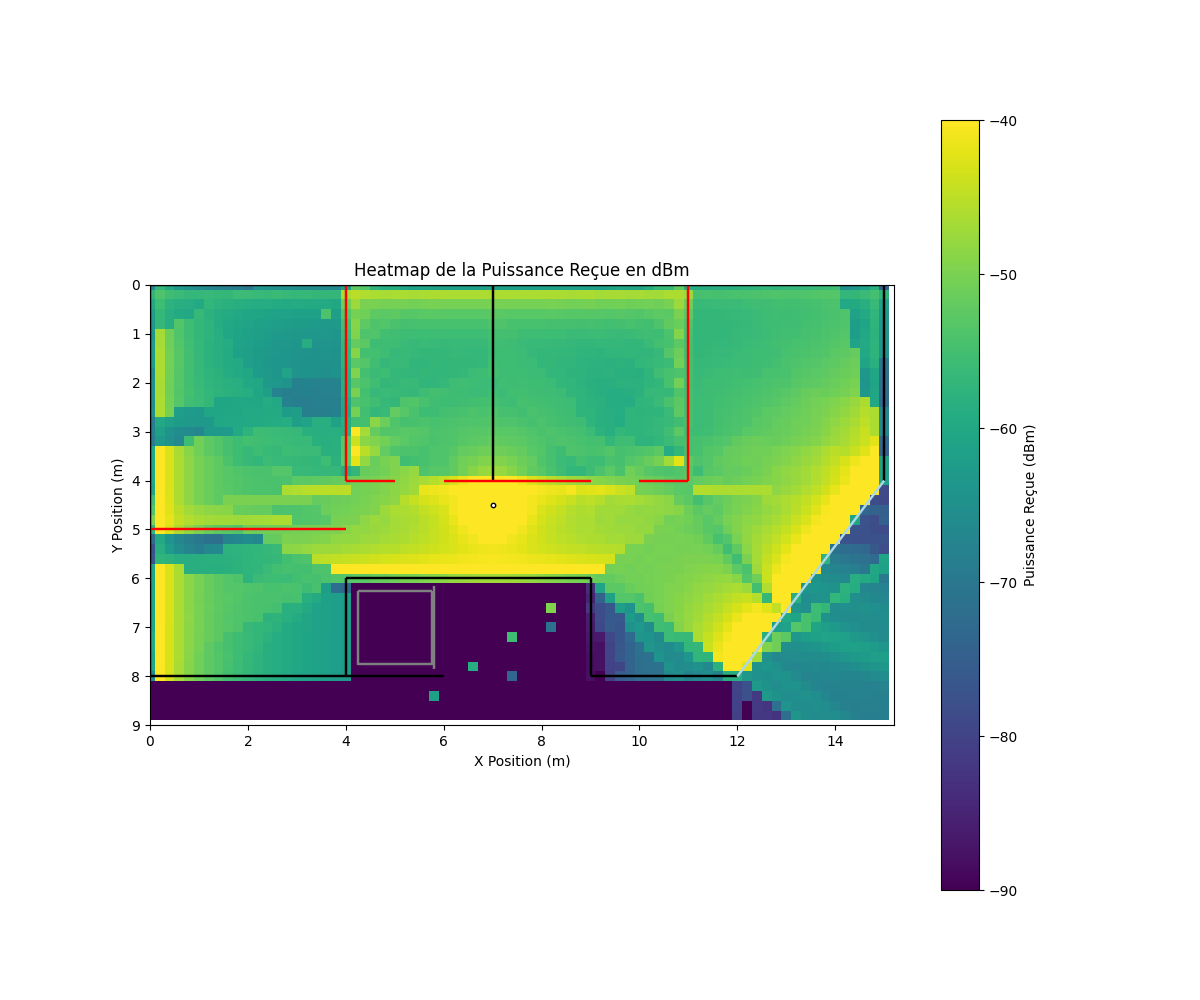
\includegraphics[width=\textwidth]{Pictures/opt1bpma.png}
    \caption{Heatmap puissance (dBm) avec ascenseur\ref{opti1adbm}}
    \label{fig:}
\end{subfigure}
\hfill
\begin{subfigure}[b]{0.48\textwidth}
    \centering
    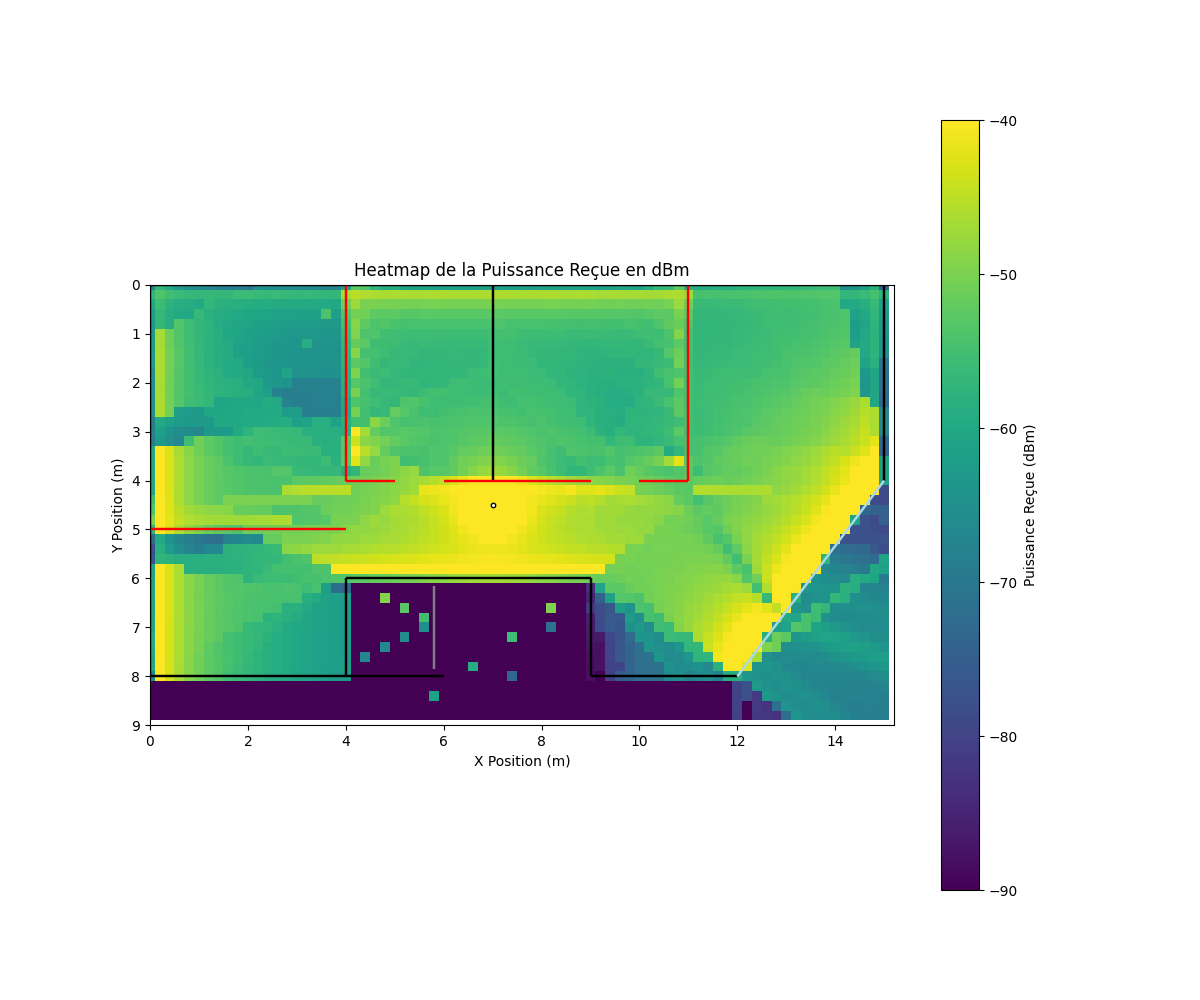
\includegraphics[width=\textwidth]{Pictures/opt1bpm.png}
    \caption{Heatmap puissance (dBm) sans ascenseur\ref{opti1dbm}}
    \label{fig:}
\end{subfigure}
\caption{Heatmaps de l'optimisation à 1 émetteur avec et sans ascenseur }
\label{okem}
\end{figure}
\subsubsection{Couverture de l'appartement à deux émetteurs}
La fonction d'optimisationà 2 émetteurs a trouvé comme positions optimales (2.5,-2.5) et (10.5,-4.5).Elles assurent une couverture totale de l'appartement dans les deux cas, que l'ascenseur soit à l'étage ou non. La puissance moyenne dans tout l'appartement reste identique dans les deux cas et est  $-48.97$ dBm. %Cependant, avoir une antenne dans sa chambre peut être dérangeant. Une optimisation sans les chambres a été faite et les positions revenues sont (4.5,-5) et (2.5,-2.5) avec une puissance moyenne de $-49.00$ dBm. Les heatmaps sont en annexe 
\begin{figure}[H]
\centering
\begin{subfigure}[b]{0.48\textwidth}
    \centering
    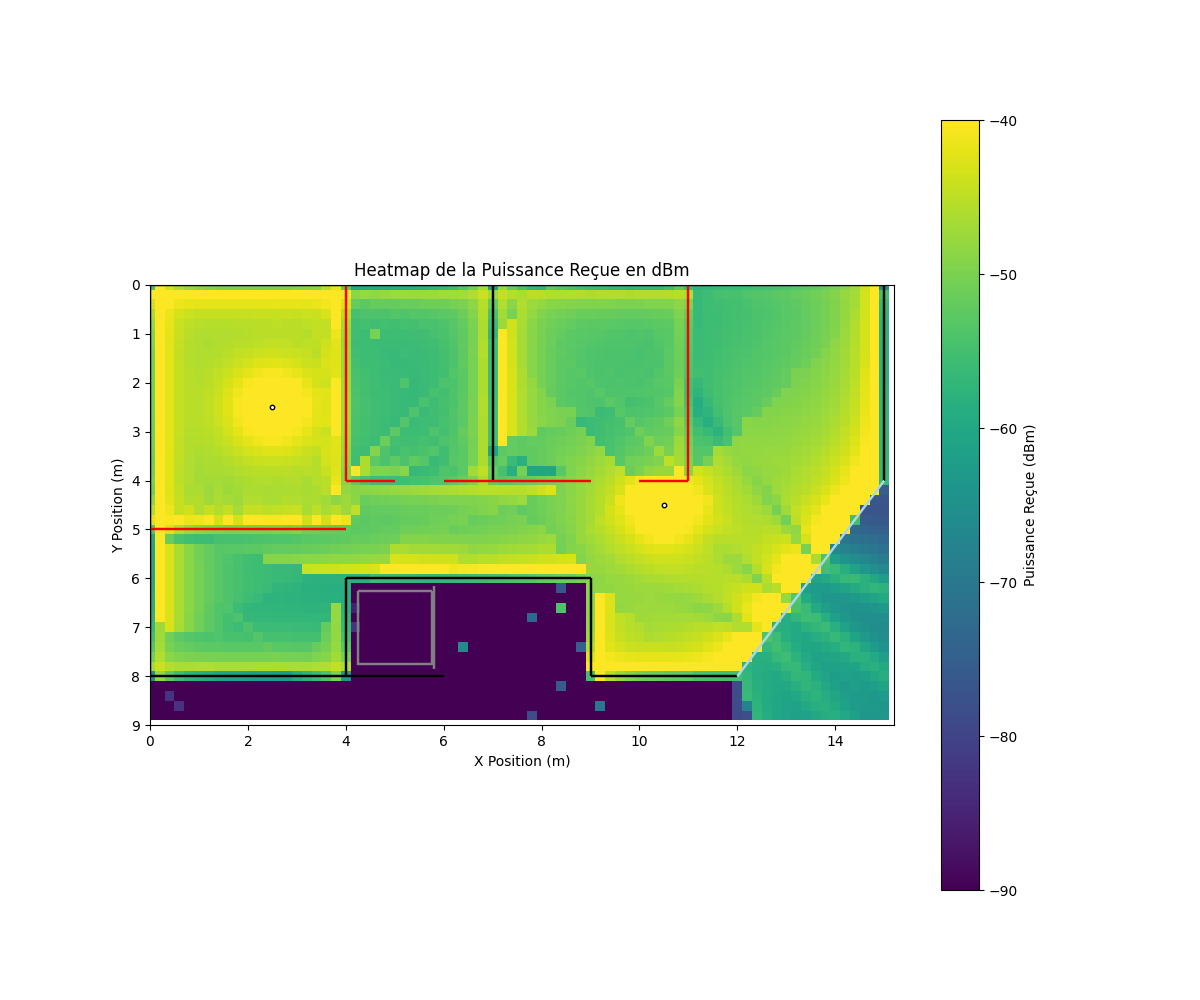
\includegraphics[width=\textwidth]{Pictures/opti2dbma.png}
    \caption{Heatmap puissance (dBm) avec ascenseur\ref{opti2dbma}}
    \label{fig:}
\end{subfigure}
\hfill
\begin{subfigure}[b]{0.48\textwidth}
    \centering
    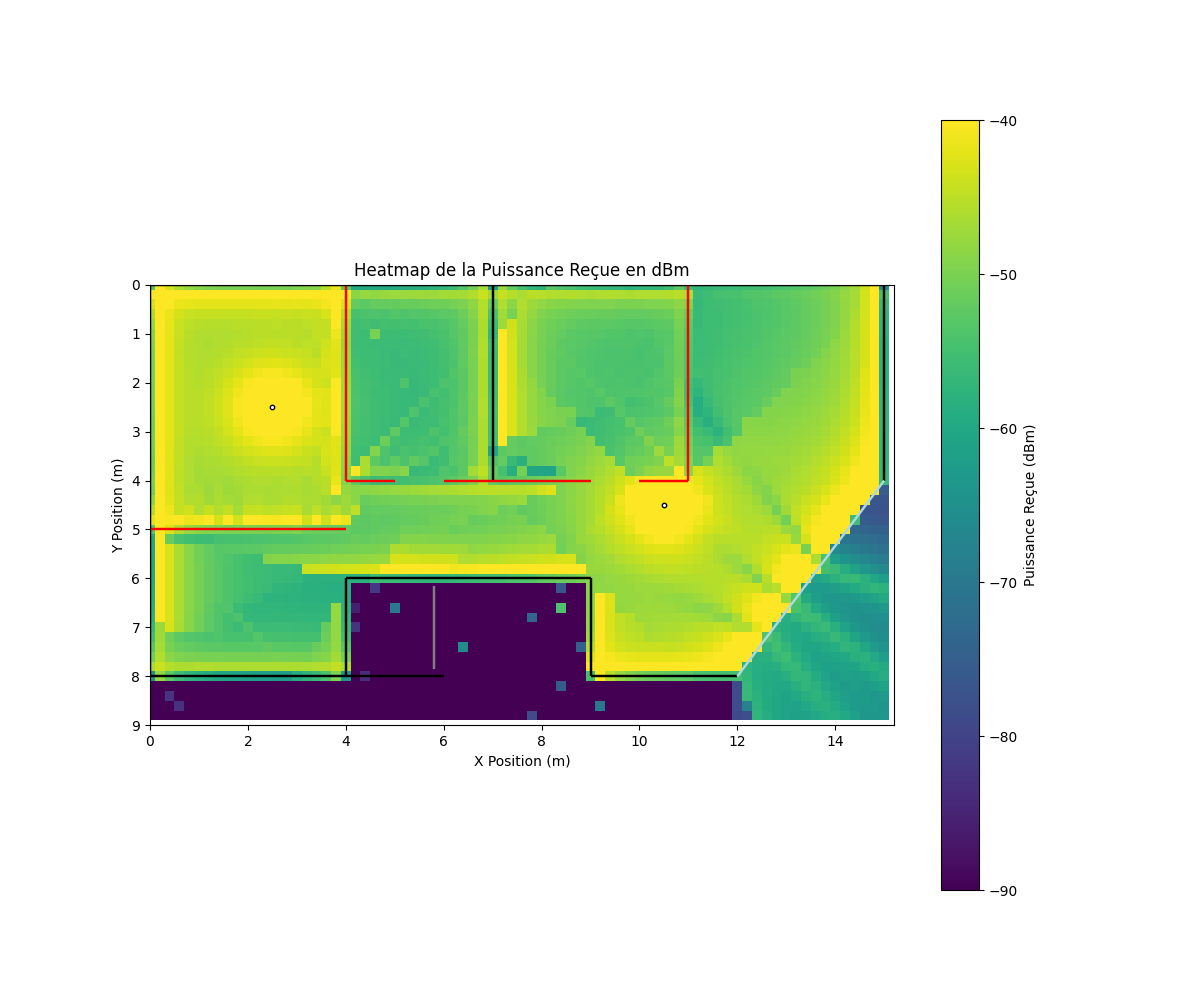
\includegraphics[width=\textwidth]{Pictures/opti2dbm.png}
    \caption{Heatmap puissance (dBm) sans ascenseur \ref{opti2dbm}}
    \label{fig:}
\end{subfigure}
\caption{Heatmaps de l'optimisation à 2 émetteurs avec et sans ascenseur }
\label{okem}
\end{figure}

L'optimisation de la position de l'émetteur est essentielle pour assurer une couverture totale de l'appartement. Il a été possible de passer de $-69,65$ dBm à $-53,08$ dBm en plaçant le même émetteur à une position optimale. % La différence de puissance de $-18,11$ dBm est considérable.
Il est également possible d'améliorer cette puissance moyenne en ajoutant des émetteurs, mais dans un cas réel cela coûterait également plus cher. Lorsque l'ascenseur est à l'étage, il est observé que aucun rayon ne traverse les parois métalliques, quelle que soit la position de l'émetteur.